\section{电功率}\label{sec:9-2}

\xiaobiaoti{电功率}
电流通过各种用电器时都做了功,但是在相等的时间里做功的多少可能相差很大。
例如,电流通过电扇的电动机,每秒钟做的功只有几十焦耳;
电流通过电车的电动机,每秒钟做的功有几万焦耳;
电流通过电力机车的电动机,每秒钟做的功达到几百万焦耳。

\textbf{电流在 1 秒钟内所做的功叫做电功率}(也常常简称为功率)。
1 秒钟内做的功越多,电功率越大。
在上段的例子里,机车电动机的电功率最大,电扇电动机的电功率最小。
如果要做同样多的功,电功率大的用的时间短,电功率小的用的时间长。
所以电功率是反映电流做功快慢的物理量。

\begin{wrapfigure}{r}{6cm}
    \centering
    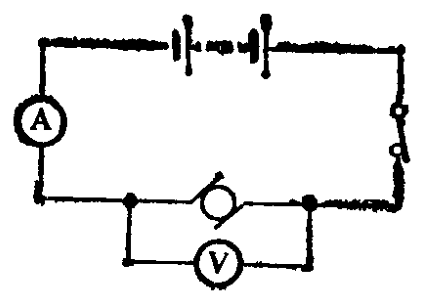
\includegraphics[width=5cm]{../pic/czwl2-ch9-2}
    \caption{}\label{fig:9-2}
\end{wrapfigure}

\begin{enhancedline}
电功率常用 $P$ 表示;因为 $P = \dfrac{W}{t}$,$W = UIt$,所以
$$ P = UI \;\juhao $$
上式表明,\textbf{电功率等于电压与电流强度的乘积}。

如果式中 $U$ 的单位用伏特,$I$ 的单位用安培, 那么 $P$ 的单位就是瓦特(简称瓦)。瓦特的符号是 W。

电功率的单位“瓦特”,也就是机械功率的单位“瓦特”,
$$ 1\wate = 1\dfrac{\jiaoer}{\miao} = 1\text{伏特·安培} \;\juhao $$
\end{enhancedline}

电功率的单位还有千瓦(kW),
$$ 1 \qianwa = 1000 \wate \;\juhao $$


既然电功率等于电压与电流强度的乘积,
我们就可以用伏特表和安培表分别测出用电器两端的电压和通过用电器的电流强度,
从而计算出用电器的电功率。
在图 \ref{fig:9-1} 所示的实验中,如果用伏特表测出电动机两端的电压是 4 伏特,
用安培表测出通过电动机的电流强度是 0.36 安培,那么,
电动机的电功率 $P = 4\fute \times 0.36\anpei = 1.44\wate$。
这个实验的电路图如图 \ref{fig:9-2} 所示。

\begin{table}[H]
    \centering
    \caption*{一些电器设备的功率}
    \begin{tblr}{lQ[r,10em]}
        半导体收音机(六管)  & 0.06 ~ 0.4 瓦特 \\
        31 厘米电视机(晶体管)  & 约 30 瓦特 \\
        日光灯  & 3 ~ 40 瓦特 \\
        电子管收音机(六灯) & 约 40 瓦特 \\
        普通家用白炽电灯  & 15 ~ 60 瓦特 \\
        常用的电烙铁 & 20 ~ 100 瓦特 \\
        碘钨灯(一般照明用)  & 1000 瓦特 \\
        韶山 I 型电力机车  & 4200 千瓦 \\
        刘家峡水电站  & 122.5 万千瓦 \\
        葛洲坝水电站  & 271.5 万千瓦 \\
    \end{tblr}
\end{table}

在电灯泡上会看到“220V \; 40W” 或 “220V \; 60W” 等字样,
在电烙铁上会看到“36V \; 100W” 或 “220V \; 50W” 等字样。
电动机铭牌上也都标着电压是多少伏特、功率是多少千瓦。

\CJKunderwave{
用电器上标着的电压值是用电器正常工作时的电压,叫额定电压。
用电器上标着的功率值是用电器额定电压时的电功率,叫额定功率}。
如果用电器两端的电压不等于它的额定电压,它的实际功率也就不等于它的额定功率。

知道了用电器的功率和使用时间,根据 $W = Pt$ 可以计算出电流所做的功。
例如, 将 “220V \; 60W” 的灯泡接在 220 伏特的电路中,通电5 小时,电流所做的功是

$ W = Pt = 60\wate \times 18000\miao = 1.08 \times 10^6\jiaoer$。

\begin{wrapfigure}[8]{r}{6cm}
    \centering
    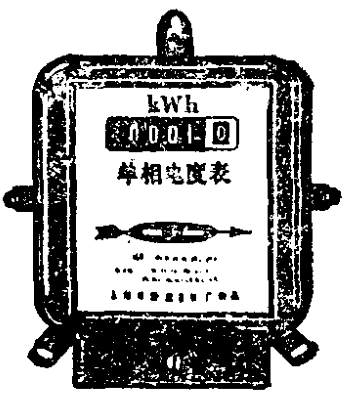
\includegraphics[width=5cm]{../pic/czwl2-ch9-3}
    \caption{电度表}\label{fig:9-3}
\end{wrapfigure}

\xiaobiaoti{千瓦时 电度表}
焦耳这个电功单位很小,用起来很不方便。
在日常用电中经常使用的电功单位是\textbf{千瓦时}(kWh)。
在电功率是 1 千瓦的时候,电流在 1 小时内所做的功,就是 1 千瓦时。
平常我们说用了几 “度” 电的 “度” 就是千瓦时。
\begin{align*}
    1\qianwashi &= 1000\wate \times 3600\miao \\
        &= 3.6 \times 10^6\text{瓦特秒} \\
        &= 3.6 \times 10^6\jiaoer \\
        &= 1\du \;\juhao
\end{align*}

前面的例子,用千瓦时做电功单位,计算起来比较方便。

$\begin{aligned}[t]
    W &= Pt = 60\wate \times 5\xiaoshi \\
      &= 0.06\qianwa \times 5\xiaoshi = 0.3\qianwashi = 0.3\du \;\juhao
\end{aligned}$

用电器用电的度数通常是由连接在电路中的电度表(图 \ref{fig:9-3})来测量的。
电度表的计数器上先后两次读数之差,就是这一段时间内的用电度数。
工农业生产上用 1 度电,电费只有几分钱,日常生活中用 1 度电,电费只有一、两角钱。
但我们绝不能因为电费便宜而浪费电。
1 度电在生产上的作用很不小呢,图 \ref{fig:9-4} 表示出了 1 度电的作用。

\begin{figure}[H]%[htbp]
    \centering
    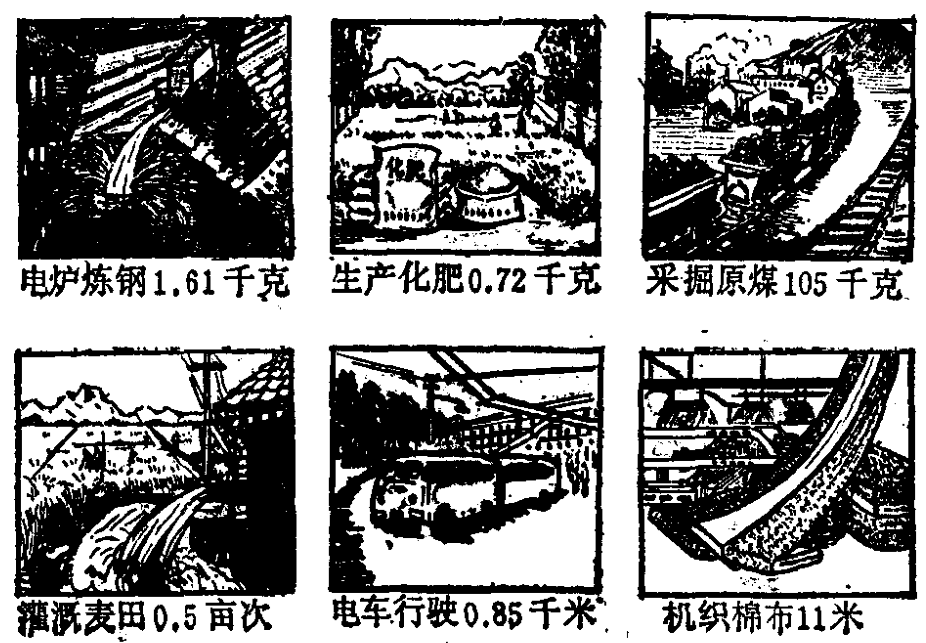
\includegraphics[width=0.8\textwidth]{../pic/czwl2-ch9-4}
    \caption{1 度电的作用}\label{fig:9-4}
\end{figure}

